\subsection{Beschaltung der Empfangsdiode}
\label{subsec:receiver_schematic}
Für die Empfangsdiode \textsc{AVAGO HFBR-2416} ist folgendes Prinzipschaltbild aus dem Datenblatt\footnote{Avago, HFBR-2416, Seite 23, Figure 12 http://docs.avagotech.com/docs/AV02-0176EN} gegeben:
\begin{figure}[H]
	\centering
	\includegraphics[scale=0.65]{gfx/hfbr.pdf}
	\caption{Prinzipschaltbild Empfangsdiode}
	\label{fig:basic_schematic} 
\end{figure}
\begin{figure}[H]
	% minipage mit (Blind-)Text
	\begin{minipage}{0.45\textwidth} 
		Die Prinzipschaltung wurde übernommen, um den Betrieb innerhalb der Spezifikationen zu gewährleisten. Die Bauteile sind so dimensioniert, dass die Grenzfrequenz des Hochpasses aus $R_4$ und $C_5$ unter dem Nachrichtensignal bei $50Hz$ liegt. Der Hochpass dient der Filterung von DC-Offsets seitens der Diode. \\ \\
	Für $R_4$ wurde $33k\Omega$ gewählt. Damit ergibt sich eine neue Grenzfrequenz von $ f_{g}=48,23Hz $.
	\end{minipage}
	% Auffüllen des Zwischenraums
	\hfill
	% minipage mit Grafik
	\begin{minipage}{0.45\textwidth}
	Berechnung des Hochpasses: \\ \\
	Mit $C_5 = 100nF$ und $f_g=50Hz$  folgt:
	\savebox\strutbox{$\vphantom{\dfrac11}$}
	\begin{align}
	  f_g &= \frac{1}{2 \pi \cdot R \cdot C}\\
		R &= \frac{1}{2 \pi \cdot f_g \cdot C}\\
		R &= \frac{1}{2 \pi \cdot 50 Hz \cdot 100nF}\\
		  &= 31,83k\Omega		 	
	\end{align}  
	\end{minipage}
\end{figure}
\noindent
\newpage
Nachfolgend die realisierte Schaltung:
\begin{figure}[htbp]
\centering
 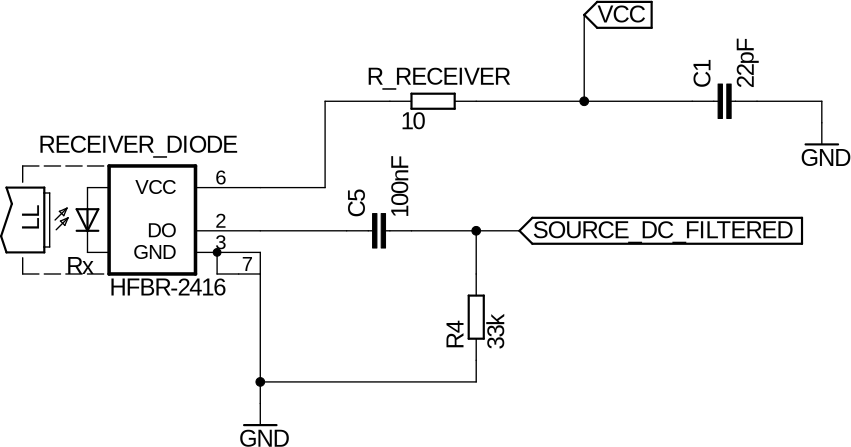
\includegraphics[scale=0.45]{gfx/receiver_part.pdf}
	\caption{Beschaltung Empfangsdiode}
\end{figure}
 
 

%\footnotetext{Quelle: Elektronik Vorlesungssunterlagen, Prof. Dr. Ralf Patz}